\chapter{Pangénomique: état des lieux, enjeux et ambitions}

 La pangénomique est un domaine d'étude en plein essor, qui a permis d'explorer et d'analyser les génomes procaryotes sous un nouveau point de vue. Mon travail de thèse s'est concentré sur l'analyse et la comparaison de pangénomes. Dans cette partie, je reviendrai d'abord sur l'origine, les concepts et les défis que pose la pangénomique.  Je présenterai ensuite les différentes modélisations permettant de représenter les génomes en pangénomique, pour poursuivre sur les méthodes de construction de pangénome. Pour terminer, je développerai les méthodes d'analyse existantes en pangénomique. Cette partie sera aussi l'occasion de faire l'état de l'art des outils en pangénomique et de présenter l'outil PPanGGOLiN sur lequel j'ai pu travailler et que j'ai utilisé dans mes développements de thèse.

\section{Origine, concept et défis}

Bien que le terme "pangénome" soit utilisé dans des articles avant 2005, en microbiologie, on s'accorde sur une origine du concept de pangénome proposé dans 2 articles fondateur \cite{medini_microbial_2005,tettelin_genome_2005}. L'idée est alors de ne pas représenter les génomes individuellement, mais d'utiliser une structure mathématique pour les représenter tous en même temps. Le pangénome représente donc l'union de toutes les séquences présente dans un ensemble de génome. Entre 2006 et 2024, ce n'est pas moins de 3 500 articles qui référencent le terme\footnote{Ce chiffre doit être revue à la baisse dû à l'utilisation erronée du terme dans certaines études et une utilisation parfois abusive pour profiter de l'intérêt croissant pour ces analyses}, dont près de 800 concernant les procaryotes (\autoref{fig:panCite}). En bioinformatique, la structure, les algorithmes, les méthodes d'analyses des pangénomes, ont constitué un nouveau champ de recherche, la pangénomique.

\begin{figure}[htbp]
    \centering
    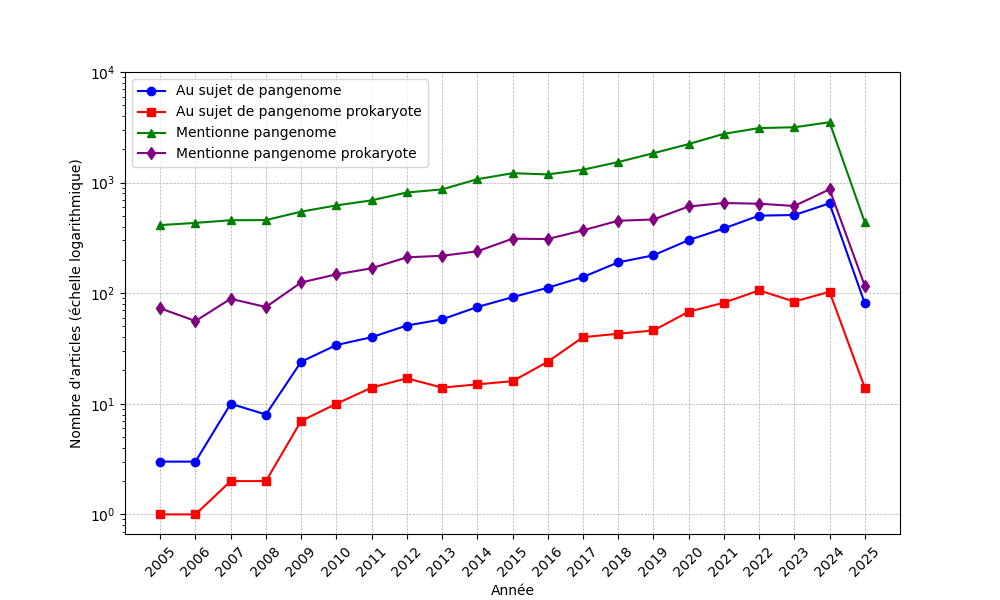
\includegraphics[width=\linewidth]{images/pangenomeCitation.png}
    \caption[Bibliométrie pangénome]{Nombre d'articles, référencé dans PubMed, par année, à propos de pangénome de 2004 au 10 février 2025. La courbe bleue représente le nombre d'articles contenant le terme pangénome dans le titre ou l'abstract : Query=("pan-genome"[Title/Abstract] OR "pangenome"[Title/Abstract] OR "pan-genome"[Title/Abstract]) AND (2004:2025[pdat]). La courbe rouge limite aux publications concernant les procaryotes : Query=("procaryote"[Title/Abstract] OR "bacteria"[Title/Abstract] OR "archeae"[Title/Abstract]) AND ("pan-genome"[Title/Abstract] OR "pangenome"[Title/Abstract] OR "pan-genome"[Title/Abstract]) AND (2004:2025[pdat]). La courbe verte représente tous les articles ou le terme pangénome est trouvé : Query=((pangenome) OR (pan genome)) OR (pan-genome) AND (2004:2025[pdat]). La courbe violette filtre les publications concernant les procaryotes : Query=(((procaryote) OR (bacteria)) OR (archeae)) AND (((pan-genome) OR (pangenome)) OR (pan genome)) AND (2004:2025[pdat]).}
    \label{fig:panCite}
\end{figure}

Le pangénome est une structure de données complexes qui peut contenir un ensemble d'informations. Notamment, à partir du pangénome, Tettelin \textit{et al.} propose de séparer les gènes en 2 catégories, les gènes "\textit{core}" commun à tous les génomes, des gènes "\textit{dispensable}" trouver dans un sous-ensemble de génomes. En généralisant, le pangénome permet de distinguer l'ensemble des séquences communes à tous les organismes, des variations présente chez certains groupes d'individus, voire spécifique à un organisme. De ce postulat a émergé l'idée de remplacer les génomes de références dans les bases de données par des pangénomes de références. Toutefois, ce changement de paradigme n'a pas encore été opéré, car il pose plusieurs questions. La première est la question de la représentation des pangénomes, nous aborderons les modèles et représentations des pangénomes, qui doit être visualisable par l'\oe il humain, tout en intégrant l'ensemble de l'information du pangénome. La seconde question est celle du stockage, les génomes sont généralement stockés sous forme de texte et relié à leurs informations dans des bases de données. Le pangénome est une structure plus complexe, qui n'est pas possible de stocker sous forme de texte. De plus, les bases de données contenant les pangénomes doivent pouvoir être interrogé de façon efficace. Étant donné l'augmentation du volume de données génomique dans les bases, il est également nécessaire que la base de données puissent être mise à jour régulièrement. La dernière question, essentiel, est : quelle méthode utiliser pour construire le pangénome ? Il faut tout d'abord définir les éléments qui constituent le pangénome, \textit{i.e.}, les gènes ou des k-mers pour les variants, ou encore des séquences d'ADN plus longues. Il faut ensuite connecter ces éléments, selon des critères pertinents. Enfin, il faut pouvoir donner un sens au pangénome et donc il faut pouvoir y appliquer des algorithmes pour l'analyser. Toutes ces questions n'ont pas encore trouvé de réponse consensus dans la communauté et aucune méthode n'a encore réussi à s'imposer comme solutions optimales. Trouvé une méthode globale est aussi un défi, car la pangénomique est appliqué dans de nombreux domaines de recherches, pour répondre à une grande diversité de question.

La pangénomique est largement utilisée dans de nombreux domaines. Le "Computational Pan-Genomics Consortium" met en avant son rôle dans le développement de solutions applicatives répondant à des problématiques communes à plusieurs disciplines \cite{the_computational_pan-genomics_consortium_computational_2018}. Elle bénéficie ainsi des avancées en phylogénie, métagénomique et intelligence artificielle.

En phylogénie, les méthodes de comparaison génomique à grande échelle et les techniques de construction d'arbres phylogénétiques ont été intégrées aux approches pangénomiques. En retour, la pangénomique permet une meilleure prise en compte des variations génétiques à l'échelle de l'ensemble des génomes, plutôt que de se limiter à un génome de référence, offrant ainsi une vision plus fine de la dynamique évolutive.

En métagénomique, les outils d’assemblage ont été adaptés pour affiner la reconstruction des pangénomes. Les algorithmes de \textit{binning}\footnote{Procédure de regroupement des contigs assemblé et d'assignation à un génome d'origine.} et de profilage génétique facilitent l’identification de clusters de gènes conservés et variables. En retour, la pangénomique enrichit l’analyse de la diversité génétique au sein des communautés microbiennes, dépassant ainsi la seule représentation de la diversité des génomes au sein d’un taxon.

L’intelligence artificielle joue également un rôle clé en améliorant l’annotation et la prédiction fonctionnelle des gènes. L’apprentissage automatique est appliqué à la pangénomique pour détecter des motifs génétiques pertinents, prédire des phénotypes et identifier des associations entre mutations et traits phénotypiques.

Ces méthodes, souvent développées pour d’autres disciplines, ont donc favorisé l’essor de la pangénomique en optimisant l’analyse des données, la reconstruction des génomes et l’interprétation des résultats.

La pangénomique se présente donc comme une solution à l'analyse de grand volume de données, à l'heure où le nombre de génomes disponible dans les banques augmentent de façon exponentielle, mais apporte aussi son lot de défis.

\subsection{Modélisation de la croissance des pangénomes}
\label{sec:croissance_pan}

Dans l'article original de Tettelin \textit{et al.}, les auteurs s'intéresse à la distribution \textit{core/dispensable} en fonction du nombre de génomes de \textit{Streptococcus agalactiae}\footnote{Bactérie du microbiote intestinale humain et animal, qui est également associé à des infections graves.} que contient le pangénome. Ils observent que lorsque le nombre de génomes augmente, la part de \textit{core genome} décroît de façon exponentielle. Ce résultat les amène à modéliser la croissance du \textit{core genomes} selon une équation exponentielle décroissante. Le modèle permet alors d'estimer la taille du \textit{core genome} pour un nombre de génomes en théorie infinie. Il est alors possible d'estimer la taille du \textit{core genome} d'une espèce à partir d'un échantillon de génome. 

À partir de ce modèle, il est également possible d'estimer la taille du pangénome, \textit{i.e.}, le nombre de gènes unique que contient le pangénome. Ils définissent alors 2 types de pangénomes en fonction de l'estimation de la taille : les pangénomes ouvert et les pangénomes fermés. Les pangénomes sont considérés comme ouverts lorsque le nombre de gènes ajouté au pangénome lors de l'ajout d'un nouveau génome, ne diminue pas avec l'ajout de nouveaux génomes. Le nombre de gènes est donc théoriquement infini pour un pangénome ouvert avec une infinité de génomes. Les pangénomes fermé quant à eux voit le nombre de nouveaux gènes progressivement diminué lors de l'ajout de nouveaux génomes. La courbe de prédiction permet d'identifier un plateau théorique du nombre maximal de familles que contiendra le pangénome avec un nombre de génomes infinis. Biologiquement, le pangénome ouvert est attendu pour les espèces sympatriques\footnote{Espèces vivant dans le même environnement que d'autres espèces.} et qui présentent un fort taux de transfert horizontaux, tandis que les espèces vivant dans des niches écologiques ou qui ont une faible capacité d'acquisition de gènes extérieurs vont avoir un pangénome fermé.

\begin{figure}[htbp]
    \centering
    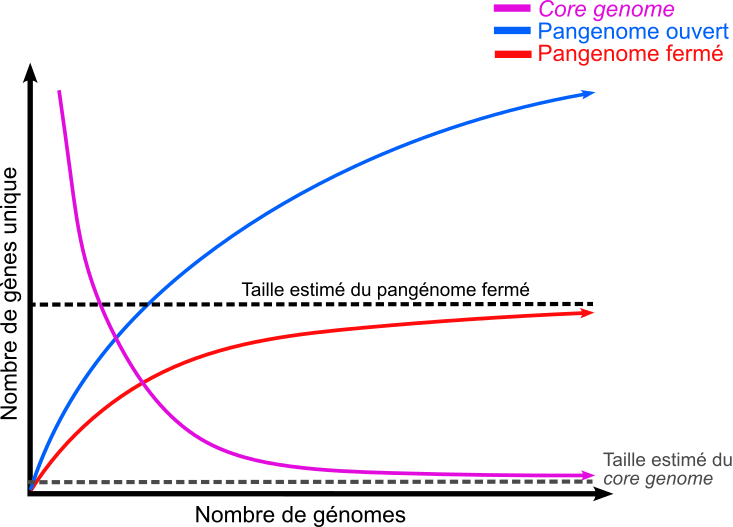
\includegraphics[width=0.7\linewidth]{images/panOpenClose.png}
    \caption[Schéma de croissance du pangénome]{Schéma de croissance du pangénome.}
    \label{fig:panOpenClose}
\end{figure}

Le modèle proposé par Tettelin \textit{et al.}, repose sur l'hypothèse que pour un nombre suffisant de génomes, le nombre de nouveaux gènes apporté par un génome devient constant à partir d'un certain nombre de génomes. Cette hypothèse implique alors que la taille du pangénome est infinie. Cette hypothèse sera questionnée par Hogg \textit{et al.} dans leur étude du pangénome de \textit{Haemophilus influenzae} \cite{hogg_characterization_2007}. Ils vont alors proposer une modélisation basée sur l'hypothèse que le pangénome est fini. Dans leur modèle, chaque gène est associé à une variable aléatoire de Bernoulli, dont la probabilité correspond à la fréquence du gène dans les génomes. Un génome est ainsi généré en observant ces variables : un gène est présent si l’essai est un succès, sinon il est absent. Bien que certains gènes ne soient pas indépendants en raison de structures comme les îlots génomiques, cette hypothèse est conservée pour simplifier le modèle. Les fréquences réelles des gènes étant inconnues, elles sont modélisées de manière probabiliste en répartissant les gènes en $K$ classes distinctes, chacune ayant une fréquence de présence spécifique. À partir de ce modèle, sur le pangénome de \textit{H. influenzae} avec $K=7$, la taille du pangénome est estimé à 5 000 gènes (contre 2 800 gènes dans les 13 génomes de bases). Ce modèle sera ensuite amélioré par Snipen \textit{et al.} \cite{snipen_microbial_2009}, qui proposeront une détermination automatique du nombre de classes $K$ et de la fréquence théorique des gènes pour chaque classe. Les modèles binomiaux propose une perspective dans laquelle la diversité en gènes est finie et qu'il existe un nombre de génomes suffisamment grand pour que tout le répertoire génique soit connu. Cette vision semble de prime abord logique, car le nombre de combinaisons possible de nucléotide ou d'acide aminé est fini. Pourtant, on peut y opposer que ce nombre, sans le calculer, semble démesuré et qu'il peut être considéré comme infini. De plus, les génomes évoluent continuellement et que de nouveaux gènes apparaissent sans cesse. L'utilisation des modèles binomiaux semble alors plus approprié à des espèces de niche, isolé et présentant un faible taux de transfert horizontaux.

En 2008, Tettelin \textit{et al.} vont proposer une nouvelle modélisation basée sur la loi de Heaps\footnote{Définit de manière empirique en linguistique, cette loi permet de décrire le nombre de mots d'une langue à partir d'un ensemble de documents.} \cite{tettelin_comparative_2008}. On estime le nombre $n$ de gènes distincts, en fonction du nombre $N$ de génomes étudiés, selon la relation :
\begin{equation}
    n=kN^\gamma, 0<\gamma<1,k\geq1
\end{equation}

Le paramètre $k$ est une constante de proportionnalité tandis que $\gamma$ reflète la tendance de la fonction. Ainsi, plus $\gamma$ est proche de 0 plus la croissance en gène distinct est lente, et plus $\gamma$ est proche de 1 plus la croissance est rapide (\autoref{fig:HeaplawGamma}).

\begin{figure}[htbp]
    \centering
    \subfloat[]{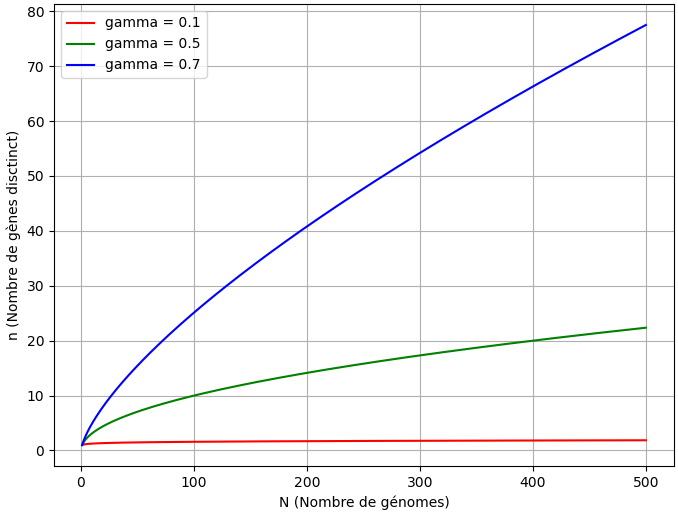
\includegraphics[width=0.48\linewidth]{images/HeapsLawgamma.png}
    \label{fig:HeaplawGamma}}
    \hfill
    \subfloat[]{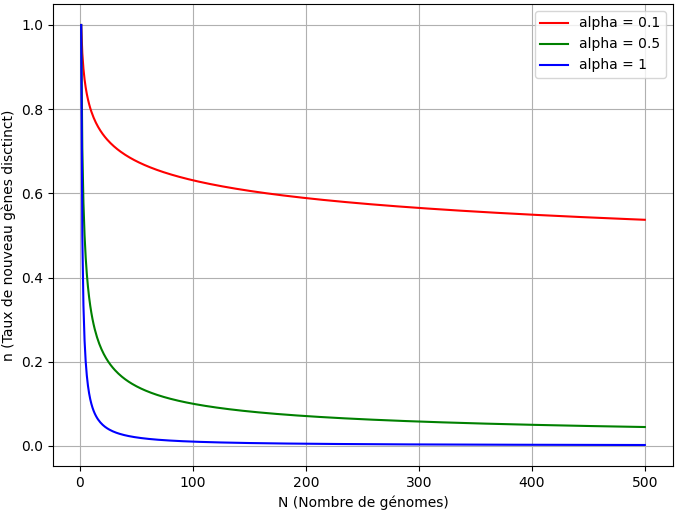
\includegraphics[width=0.48\linewidth]{images/HeapsLawAlpha.png}
    \label{fig:HeaplawAlpha}}
    \caption{Caption}
    \label{fig:Heaplaw}
\end{figure}

Selon la loi de Heap, le nombre de nouveau gènes découvert diminue à mesure que l'on ajoute des génomes. On peut formuler ceci selon l'équation : 

\begin{equation}
    p(n)=kN^{(\gamma-1)}=kN^{-\alpha}, \alpha=1-\gamma
\end{equation}

Ainsi, sur la \autoref{fig:HeaplawAlpha}, lorsque $0<\alpha<1$, le taux de nouveaux gènes décroit en ajoutant des génomes, sans jamais être nulle. Dans ce cas, le nombre de gènes distinct est croissant. Ce qui implique que si $0<\alpha<1$, le pangénome est ouvert. À partir d'un ensemble de génome, il est possible d'estimer k et $\alpha$ (ou $\gamma$) et donc de caractériser si le pangénome est ouvert. Si $\alpha\geq1$, alors le taux de nouveaux gènes atteint 0, ce qui correspond à un pangénome fermé. 

\subsection{Les différents types de pangénomes}

Les pangénomes peuvent être divisés en 2 catégories en fonction de l'unité choisit pour les construire. Le premier type, celui présenté par Tettelin \textit{et al.} \cite{tettelin_genome_2005}, utilise les gènes comme unité de base du pangénome (\autoref{fig:panType}.B). En regroupant les gènes par homologie (appelé famille de gènes, cf. \autoref{sec:fam}), il est possible d'obtenir la présence/absence de gènes similaire dans les génomes. Ces pangénomes ont l'avantage d'être moins couteux en ressources de calcul pour être construit. De plus, ils sont faciles à interpréter, car les gènes sont des unités déjà bien définies et parfois, ils sont même annotés fonctionnellement. Néanmoins, en utilisant les gènes, la méthode d'annotation à un impact important sur le pangénome et il est sensible aux erreurs d'annotation. De plus, les régions non codantes ne sont pas prises en compte dans cette approche. Enfin, les SNPs peuvent passer inaperçu après le regroupement, ainsi que les variants structuraux (SV).

L'autre type de pangénome est basé sur les séquences brutes des génomes. Cette approche plus récente, qui peut être associé à l'outil GenomeMapper \cite{schneeberger_simultaneous_2009}, permet d'identifier les parties similaires des parties variables à partir d'un alignement complet des séquences découpé en k-mers (\autoref{fig:panType}.C,D). Cette approche a l'intérêt de prendre en compte toute la diversité des génomes (codant, non codant, SNPs et SV). Toutefois, la construction de ces pangénomes est plus coûteuse en ressources. De plus, l'interprétation est plus complexe, car le pangénome n'est pas annoté au départ. Pour terminer, certaines méthodes de construction, utilise un génome de référence comme séquence de base (\autoref{fig:panType}.C), ce qui peut aussi introduire un biais.

\begin{figure}[htbp]
    \centering
    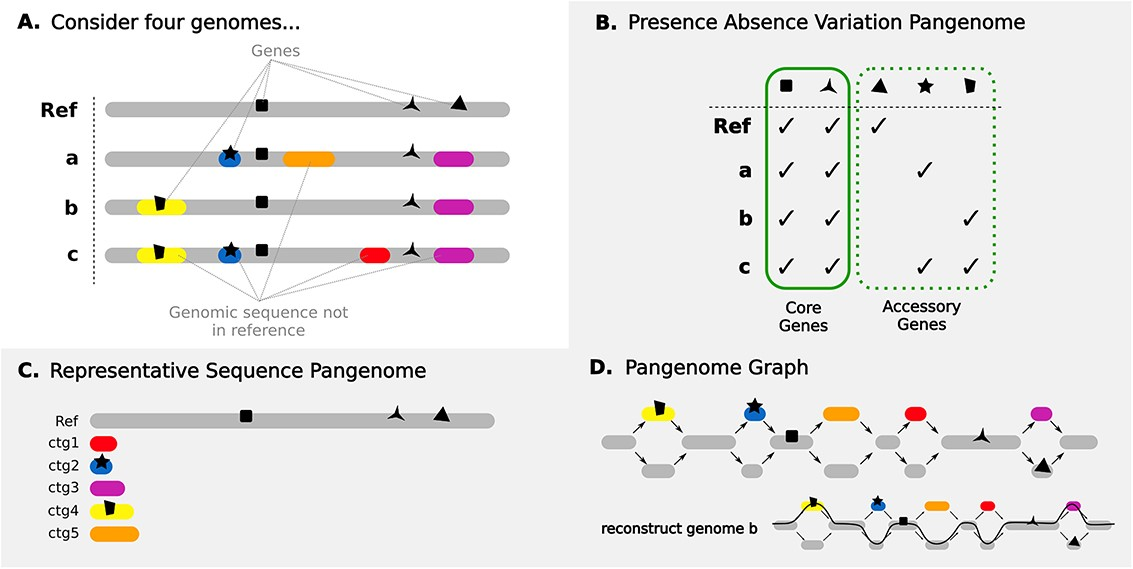
\includegraphics[width=0.8\linewidth]{images/pangenomeTypes.jpeg}
    \caption[Différents types de pangénomes]{Différents types de pangénomes. Extrait de \cite{matthews_gentle_2024}}
    \label{fig:panType}
\end{figure}

\newpage
\section{Pangénome de séquences}

\subsection{Pangénome basé sur une séquence représentative}

Un pangénome basé sur les séquences correspond à un ensemble de génomes dont l'alignement minimise le nombre de régions homologues tout en rendant compte de toute la diversité. L'objectif derrière ces pangénomes est d'obtenir une séquence pangénomique de référence. De façon contre-intuitive (par rapport à la définition "sans-référence" des pangénomes), pour construire ces pangénomes, on utilise une séquence représentative comme base. Toutes les séquences seront alignées à partir de cette base, et les segments non redondants détectés dans au moins un génome seront intégrés à la référence non redondante (NRR, Non-Redundant Reference en anglais). L'ensemble, séquence représentante et NRRs, forme alors la séquence pangénomique de référence.

\subsubsection{Méthode de construction}

Pour construire ces pangénomes, il faut d'abord identifier une séquence représentative. Les autres séquences, en général des séquences non assemblées (lectures ou \textit{reads} en anglais), sont alignées contre la représentante et les séquences non alignables sont considérées comme des NRRs potentiels. Les NRRs de taille inférieure à 500 pb sont exclues, ainsi que celles dont la similarité avec la représentante est supérieure à un seuil (90 \% en général). Les NRRs restantes sont comparées à des bases de données pour retirer tous les contaminants potentiels. De ce schéma général, on peut identifier 4 méthodes différentes pour l'identification des NRRs potentiels :
\begin{itemize}
    \item \textbf{Assemblage de type métagénomique} : les lectures non alignées sur la référence sont regroupées et assemblées \textit{de novo}. Les contigs obtenus sont ajoutés à la séquence représentante. Cette méthode est efficace même avec une faible couverture des lectures.
    \item \textbf{Assemblage itératif} : Dans un premier temps, les lectures non alignées du premier échantillon sont assemblées et ajoutées au génome de référence. Ce génome mis à jour sert ensuite de base pour l’assemblage des échantillons suivants. Ce processus est répété pour tous les échantillons.
\end{itemize}
\newpage
\begin{itemize}
    \item \textbf{Assemblage indépendant des \textit{reads} non alignés} : Toutes les lectures non alignées sont séparées par échantillon\footnote{Ensemble de lectures obtenues simultanément} et assemblées \textit{de novo} indépendamment. Les contigs obtenus sont regroupés selon leur similarité. Dans chaque groupe, un contig référent est identifié et est intégré à la séquence référente. Cette méthode nécessite une couverture d’au moins 10×, pour obtenir des contigs de taille suffisante.
    \item \textbf{Assemblage génomique indépendant} : chaque échantillon est assemblé indépendamment, et les contigs obtenus sont alignés à la référence. Les contigs non alignés sont regroupés par similarité et un contig référent est ajouté à la séquence référente.
\end{itemize}

Le choix de la méthode dépend du type et de la quantité des données disponibles. Avec une faible couverture (<10×) et un grand nombre d’échantillons, l’approche métagénomique est recommandée, bien qu’elle puisse produire des contigs chimériques. Avec une couverture plus élevée (>10×), l’assemblage indépendant ou l’approche itérative sont préférables. Cette dernière est plus lente, mais facilite l’ajout de nouveaux échantillons. Enfin, si plusieurs assemblages de haute qualité existent déjà, l’assemblage génomique indépendant est la meilleure option. Ces méthodes peuvent être combinées pour optimiser l’utilisation des données disponibles.
 
\subsubsection{Domaines d'application des pangénomes basés sur une séquence représentative}

Ces pangénomes sont particulièrement utiles lorsque les données de départ sont des \textit{lectures}. En utilisant ces modèles, il est possible de revenir à une séquence linéaire qui peut être utilisée dans les outils classiques de génomique. De plus, il peut également être utilisé comme étape préliminaire à la construction d'autres types de pangénomes, en réduisant rapidement la redondance dans un sous-ensemble proche de génomes. 

L'outil NGSPanPipe \cite{kulsum_ngspanpipe_2018} est un pipeline intégré conçu pour l'identification du pangénome à partir de lectures courtes (short reads) issues du séquençage de nouvelle génération (NGS). Contrairement à d'autres méthodes nécessitant des prétraitements des lectures, NGSPanPipe permet une analyse directe des reads bruts pour identifier le pangénome. Il ne génère pas de séquence pangénomique linéaire, mais il permet de reconstruire des contigs à partir des lectures en utilisant un génome de référence. Les contigs obtenus à partir des lectures alignées, permettent de calculer la couverture du génome par rapport au pangénome. Les lectures non alignées sont comparées à des bases de données de \textit{reads} pour identifier de nouveaux \textit{reads}, puis ils sont assemblés en contigs. L'ensemble des contigs (de lectures alignées et non alignées) sont annotés et utilisés pour construire une matrice binaire représentant la présence ou l'absence des gènes dans la séquence de référence.

\subsection{Pangénome graphe}

Les graphes de séquences sont un modèle de pangénome permettant de visualiser la diversité génomique, qu’elle soit basée sur une séquence de référence ou non. Dans tous les cas, des segments de séquences vont constituer les n\oe uds du pangénome et les arêtes seront étiquetées par des informations permettant de retrouver le lien entre les segments (comme l'organisation dans les génomes). Ce modèle pangénomique a l'intérêt de représenter toute la diversité, codant et non codant. 

\subsubsection{Méthodes et outils de construction}

\paragraph{Graphe de variant prédéterminé}

La première méthode de construction des graphes de pangénome se base sur l'utilisation d'une séquence référente et d'un fichier contenant les variations connues dans les autres séquences par rapport à cette référence. Cette méthode a l'intérêt de demander peu de ressources, car les variations sont prédéterminées et données en entrée. Toutefois, pour obtenir un graphe fiable et précis, un génome complet de bonne qualité est requis.

L'outil VG (\textit{Variation Graph toolkit}) \cite{garrison_variation_2018}, contient un ensemble d'outils permettant de générer un graphe de variants. À partir de ce graphe, qui peut être assimilé à un graphe de pangénome, il est possible de détecter les variants structuraux (SVs) et les SNPs rapidement. Le graphe est indexé, rendant les recherches et l'alignement plus efficaces, notamment dans l'alignement de lectures ou dans la recherche de variants génétiques (\textit{variant calling}). L'outil a d'abord été développé pour la génomique humaine, mais il est tout à fait possible de l'utiliser avec des génomes procaryotes.

L'outil Minigraph \cite{li_design_2020}, lui aussi développé pour le variant calling sur le génome humain, propose une méthode demandant moins de ressources que VG. Le graphe est plus léger, sans annotation, permettant de construire des graphes de pangénome de grande taille, en utilisant peu de mémoire de calcul et de stockage. Minigraph permet de capturer les grandes variations génomiques, mais est moins performant sur la détection des SNPs par rapport à VG.

\paragraph{Graphe d'alignement multiple}

Une méthode, proche de la précédente, est celle basée sur l'alignement multiple des séquences (MSA\footnote{cf. \autoref{paragraph:MSA}}) entre elles. Cette méthode n'est pas dépendante d'une séquence référente. Le MSA permet de déterminer les variations entre les séquences, ce qui augmente le coût en ressources par rapport au graphe de variants prédéterminé. Toutefois, cette méthode est plus adaptée dans le cas où plusieurs séquences de bonne qualité sont disponibles pour construire le pangénome. En effet, le MSA permet de se passer du biais de la séquence référente dans la construction du graphe et d'ainsi mieux représenter la diversité génomique.

L'outil Harvest \cite{treangen_harvest_2014}, permet de comparer des génomes étroitement apparentés. Pour optimiser l'étape d'alignement, il utilise l'outil progressiveMauve \cite{darling_progressivemauve_2010}, qui fait un alignement progressif des séquences. Après l'alignement, il identifie le \textit{core genome} dans le pangénome et génère une phylogénie basée sur une matrice des SNPs. Bien qu'étant rapide et efficace, il n'est pas adapté aux génomes très divergents et il ne permet pas d'analyser les éléments mobiles (MGE).

PGGB \cite{garrison_building_2024}, utilise des algorithmes de graphes de préfixes minimaux (MPHF\footnote{Minimal Perfect Hash Function (MPHF) est une fonction qui associe de manière unique chaque élément d’un ensemble sans collisions et avec un espace mémoire minimal}), pour compresser le graphe et optimiser l'alignement. Il est capable d'identifier et de représenter les SNPs, SV, et les MGEs de manière efficace. PGGB est conçu pour mener des études pangénomiques à grande échelle, prenant en compte de grandes quantités de séquences, ce qui demande des ressources disponibles importantes. De plus, c'est un outil assez complet pour les analyses, ce qui peut le rendre difficile d'accès.

\paragraph{Graphe de De Bruijn}

Les graphes de De Bruijn (De Bruijn Graph : DBG) sont des graphes orientés dont les n\oe uds représentent des k-mers et les arêtes le chevauchement entre le suffixe et le préfixe (de taille k-1) des k-mers (\autoref{fig:deBruijn}). Ainsi, en suivant un chemin, il est possible de reconstituer une séquence. C'est pourquoi les DBG sont utilisés dans de nombreuses applications en bioinformatique (assemblage, correction des erreurs de séquençage, métagénomique\dots) et notamment en pangénomique.

\begin{figure}[htbp]
    \centering
    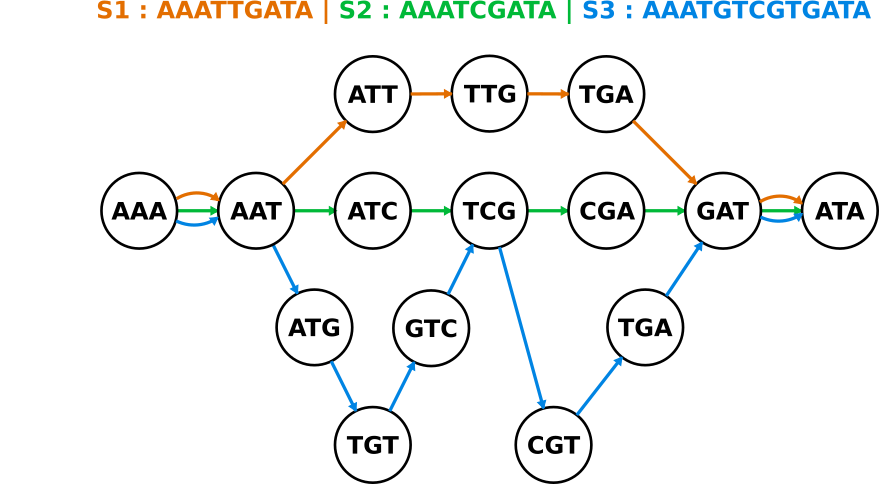
\includegraphics[width=.9\linewidth]{images/DBG.png}
    \caption[Exemple d'un graphe de De Bruijn]{\textbf{Exemple d'un graphe de De Bruijn.} Ici $k=3$, ce graphe permet de représenter et de reconstruire 3 séquences.}
    \label{fig:deBruijn}
\end{figure}

Les DBG, permettent d'avoir une structure compacte des séquences du pangénome. Les n\oe uds et les arêtes sont colorées en fonction des génomes dans lesquels ils sont retrouvés. Les DBG peuvent être compactés en cDBG, en fusionnant chaque région \textit{core}, \textit{i.e.} chaque suite de n\oe uds avec une seule arête entre chaque n\oe ud. Ces nouveaux n\oe uds fusionnés sont appelés "\textit{unitig"} et seront étiquetés avec la séquence combinée des k-mers.

L'une des premières méthodes développées utilisant des DBG est la méthode Cortex \cite{iqbal_novo_2012}, qui construit un DBG "coloré" (les arêtes et les n\oe uds sont étiquetés par les échantillons dans lesquels ils sont trouvés). À partir de ce DBG coloré, il est possible d'identifier les variants et de les associer à un génotype. Des outils plus récents, comme Bifrost \cite{holley_bifrost_2020}, améliorent les méthodes de coloration de DBG, permettant d'augmenter le volume de données pris en compte et supportant la mise à jour du graphe. Les auteurs de Bifrost ont notamment appliqué leur méthode sur une collection de plus de 100 000 génomes de \textit{Salmonella} \cite{luhmann_blastfrost_2021}, leur permettant d'identifier des gènes reliés à des îlots de pathogénicité et à une résistance aux fluoroquinolones\footnote{Classe d'antibiotique utilisée pour traiter les infections bactériennes graves.}.

\newpage
SplitMEM \cite{marcus_splitmem_2014}, permet de construire rapidement et efficacement des cDBG en intégrant une méthode appelée "saut de suffixe"\footnote{Le cDBG est relié à des arbres de suffixes, un saut de suffixe permet depuis un suffixe à l'extrémité d'une branche de l'arbre de sauté vers un même suffixe plus proche de la racine. Les sauts se poursuivent jusqu'à atteindre le suffixe le plus proche de la racine. Le chemin restant correspond au chemin le plus court sans ramification, entre la racine et le suffixe.}, qui permet de construire le cDBG sans passer par un DBG. L'outil permet ensuite de détecter dans l'ensemble des génomes ou dans un sous-ensemble de génomes les régions compressées (appelées \textit{Maximum Exact Matches} : MEMs), correspondant au \textit{core genome}. Cet outil est linéaire en temps et en espace pour identifier le \textit{core genome}, mais ne permet pas de mener d'autres analyses. De plus, la méthode a été testée sur un jeu de 62 génomes de \textit{E. coli}, le caractère linéaire est donc à vérifier sur de plus grands jeux de données.

PanTools \cite{sheikhizadeh_pantools_2016}, est un outil complet qui a largement évolué depuis sa publication. Il permet la construction de pangenomes basés sur des cDBG généralisés. PanTools est robuste à l'utilisation de grands volumes de données, que ce soit en temps, en mémoire ou en stockage. Il intègre également des méthodes d'annotation structurale et fonctionnelle, de partitionnement, d'alignement, de phylogénie, d'identification du \textit{core genome} et de visualisation. 

DBGWAS \cite{jaillard_fast_2018}, construit également les pangénomes avec des cDBG. Son originalité réside dans l'association de phénotypes (\textit{Genome Wild Association Study} : GWAS). L'intérêt d'utiliser le graphe de pangénome est qu'il n'est pas nécessaire d'utiliser une séquence de référence, contrairement aux approches classiques de GWAS. De plus, les phénotypes ne sont pas associés à des SNPs mais à des sous-graphes, permettant d'extraire des variants plus longs ou plus complexes. DBGWAS intègre une partie visualisation, permettant d'explorer les variants associés au phénotype dans leur contexte génomique pour identifier des régions variables plus larges comme les îlots génomiques. 

Le DBG (et ses dérivés) est une structure de données puissante, permettant de calculer, analyser et stocker, rapidement et efficacement, de grandes quantités de données. Néanmoins, ce qui fait la force de cette approche (l'utilisation de k-mer) est aussi sa faiblesse. Le choix de la taille du k-mer va influencer le graphe et donc la découverte des variations. De plus, cette structure est limitée dans l'identification et l'étude des régions répétées. C'est pourquoi des auteurs proposent des méthodes pour lier des informations au DBG \cite{turner_integrating_2018}.

\subsubsection{Application des graphes de pangénome.}

L'utilisation de pangénomes de séquence est très utile à partir de lectures courtes pour améliorer le génotypage. En utilisant le pangénome, contenant des variants connus, on améliore la couverture des lectures et donc on améliore le génotypage de ces lectures. Par rapport aux méthodes utilisant un génome de référence, le pangénome réduit le biais en faveur de la séquence de référence, particulièrement pour les grandes insertions/délétions et les SV. Le pangénome améliore aussi le \textit{variant calling} (VC) en augmentant sa précision, et à partir des DBG de faire du VC sans référence.

Les graphes de séquences sont également utilisés en métagénomique. L'outil MetaKallisto \cite{schaeffer_pseudoalignment_2017} utilise notamment une base de données de séquences représentantes qu'il représente sous forme de DBG coloré afin de faire de l'assignation taxonomique et de la quantification de séquences métagénomiques.

L'utilisation des graphes de séquences pour les GWAS permet de détecter finement des variations dans les populations associées à un phénotype. Chaguza \textit{et al.} \cite{chaguza_bacterial_2020} ont mené une étude sur 909 échantillons de souche hyper virulente de \textit{Streptococcus pneumoniae} (serotype 1). Ils ont pu identifier, grâce à l'outil DBGWAS, des mutations de certaines protéines associées à des phénotypes spécifiques (âge de l'hôte, géographie, structure des populations\dots). L'utilisation de graphes de pangénome a permis de mener une étude à large échelle, tout en prenant en compte toute la diversité sans nécessiter de référence.

\begin{table}[htbp]
    \centering
    \begin{tabular}{|p{.25\textwidth}|p{.3\textwidth}|p{.35\textwidth}|}
        \hline
        Nom & Méthode & Référence \\
        \hline
        NGSPanPipe & Séquence représentative & \cite{kulsum_ngspanpipe_2018} \\
        \hline
        Spine & Séquence représentative & \cite{ozer_characterization_2014}\\
        \hline
        VG toolkit & Variant prédéterminé & \cite{garrison_variation_2018} \\
        \hline
        Minigraph & Alignement sur graphe & \cite{li_design_2020} \\
        \hline
        PanVC & Variant prédéterminé & \cite{norri_founder_2021} \\
        \hline
        Minigraph-Cactus & MSA & \cite{hickey_pangenome_2024}\\
        \hline
        Harvest & MSA & \cite{treangen_harvest_2014} \\
        \hline
        PGGB & MSA & \cite{garrison_building_2024}\\
        \hline
        Cortex & graphe de De Bruijn & \cite{iqbal_novo_2012} \\
        \hline
        Bifrost & graphe de De Bruijn & \cite{holley_bifrost_2020} \\
        \hline
        SplitMEM & graphe de De Bruijn & \cite{marcus_splitmem_2014} \\
        \hline
        PanTools & graphe de De Bruijn & \cite{sheikhizadeh_pantools_2016} \\
        \hline
        twoPaCo & graphe de De Bruijn & \cite{minkin_twopaco_2017}\\
        \hline
        DBGWas & graphe de De Bruijn & \cite{jaillard_fast_2018}\\
        \hline
        PanVA & Visualisation & \cite{van_den_brandt_panva_2024} \\
        \hline
    \end{tabular}
    \caption[Outils de pangénomique basés sur les séquences]{\textbf{Liste non exhaustive d'outils de pangénomique basés sur les séquences.}}
    \label{tab:pangenomicToolsSeq}
\end{table}
\newpage
\section{Pangenome de gènes}

\subsection{Généralités et concepts}

Les outils basés sur des pangénomes de gènes, aussi appelés \textit{Presence-absence variation pangenome}s (en anglais, PAV), représentent une grande part des outils de pangénomique procaryote. Le génome des procaryotes étant majoritairement codant, et ce type de pangénome étant plus facile à manipuler et à interpréter, de nombreuses études utilisent les gènes comme unité pour construire les pangénomes. Pour construire ces pangénomes, on commence par regrouper les gènes en familles de gènes, puis on partitionne\footnote{N.B : Dans la suite, pour ne pas faire de confusion entre le partitionnement des familles et le partitionnement des gènes en famille de gènes, nous utiliserons le terme clustering pour parler de la construction des familles de gènes.} les familles en fonction de leur présence dans les génomes (\textit{core}, \textit{accessory}\dots).

% \newpage
\paragraph{Construction des familles de gènes}

La construction des familles de gènes consiste à appliquer une méthode de clustering des gènes par similarité, que nous avons vue en \autoref{sec:clustering}. Le choix de la méthode et des seuils appliqués dans le clustering auront un impact important sur le pangénome. L'outil de clustering influencera aussi l'interprétation. Tout d’abord, les outils d’analyse peuvent s’appuyer sur différents niveaux d’information, tels que la séquence nucléotidique ou protéique, la structure tridimensionnelle des protéines ou encore la fonction biologique associée. Le choix de cette base de comparaison influence de manière déterminante le calcul de la similarité, et par extension, l’inférence du caractère homologue. De plus, en utilisant un outil qui construit des clusters (et donc des familles) d'orthologues, comme orthoMCL \cite{li_orthomcl_2003} ou la base de données COG (cluster of orthologous genes), on retrouvera dans la même famille les gènes ayant suivi les mêmes événements de spéciation. Si l'outil permet de différencier les paralogues des orthologues comme InParanoïd \cite{remm_automatic_2001}, il y aura plus de familles que si on prenait en compte uniquement l'homologie. Le choix de la méthode de clustering est donc essentiel.

\paragraph{Partitionnement du pangénome}

Une fois que les génomes ont été annotés et les familles de gènes construites, les familles de gènes sont partitionnées en fonction de leur présence/absence dans les génomes. Dans les premières analyses, les familles étaient séparées en 2 parties (\autoref{fig:pangenome2}), les familles qui sont présentes dans tous les génomes sont dites "c\oe ur" (\textit{core} en anglais) et les autres sont dites "accessoire" (\textit{accessory} ou \textit{dispensable} en anglais). Cette dichotomie en \textit{core genome} et \textit{accessory genome} est liée au caractère essentiel ou non des fonctions codées par les gènes. Les familles "\textit{core}" sont impliquées dans les processus cellulaires vitaux, ce qui crée une forte pression de sélection de leurs gènes et une forte conservation dans l'ensemble des génomes. À l'inverse, les familles accessoires sont plutôt liées à des adaptations à l'environnement, à un mode de vie\dots. Leurs gènes sont donc moins soumis à la pression de sélection et donc moins conservés dans les génomes.

\begin{figure}[htbp]
    \centering
    \subfloat[Pangénome bipartie]{
        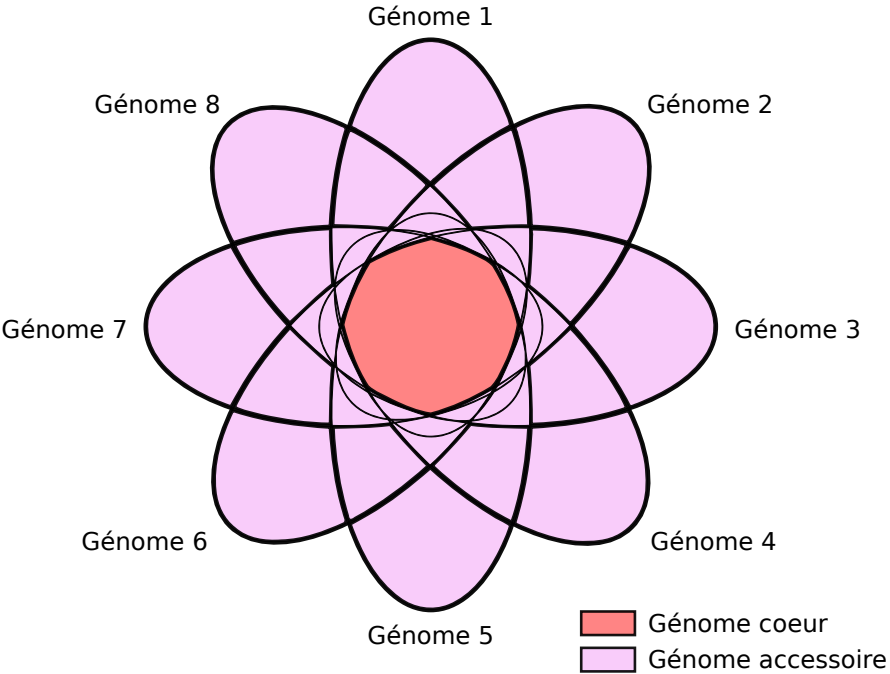
\includegraphics[width=0.48\linewidth]{images/pangenome2.png}
        \label{fig:pangenome2}
    }
    \hfill
    \subfloat[Pangénome tripartie]{
        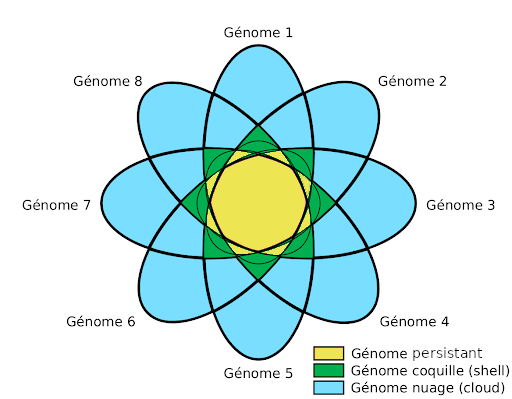
\includegraphics[width=0.48\linewidth]{images/pangenome3.png}
        \label{fig:pangenome3}
    }
    \caption[Partitionnement des pangénomes.]{\textbf{Partitionnement des pangénomes.} Extrait et adapté de \cite{gautreau_conceptualisation_2020}}
    \label{fig:pangenomeVenn}
\end{figure}

\newpage
Ce partitionnement du pangénome en 2 parties, bien que largement utilisé, est une vision très limitée de la distribution des gènes dans les génomes, qui peut amener à des erreurs d'interprétation. Il faut d'abord prendre en compte que même si le nombre de génomes disponibles est de plus en plus conséquent, il n'est toutefois pas possible d'avoir l'ensemble des génomes d'une espèce (cf. \autoref{sec:croissance_pan}), ce qui implique qu'il est plus que probable que des gènes soient identifiés comme accessoires alors qu'ils sont \textit{core} et inversement. 
De plus, les techniques de séquençage et les outils bioinformatiques ne sont pas infaillibles, et donc une erreur d'assemblage, d'annotation, de regroupement en familles, ou encore l'utilisation de génomes partiels, peut entraîner le mauvais classement d'une famille. Pour répondre à ce problème, Lapierre et Gogarten \cite{lapierre_estimating_2009} suggèrent de définir un c\oe ur relâché (\textit{soft-core} en anglais), qui contient les familles présentes dans 95 \% des génomes\footnote{ce pourcentage peut varier en fonction des études.}. Une autre proposition, de Snippen \textit{et al.} \cite{snipen_microbial_2009} raffinant un modèle proposé par Hogg \textit{et al.} \cite{hogg_characterization_2007}, rendrait le nombre de partitions variable en fonction du contenu du pangénome. Cette dernière proposition permet de ne pas utiliser de seuil fixe pour partitionner les familles.
En parallèle, Koonin \textit{et al.}, dans une analyse de l'ensemble des génomes procaryotes disponibles en 2008 \cite{koonin_genomics_2008}, et Makarova \textit{et al.}, en étudiant l'ensemble des génomes d'archées disponibles en 2007 \cite{makarova_clusters_2007}, proposent une vision tripartie du pangénome (\autoref{fig:pangenome3}). Les 2 articles suivent une méthodologie similaire : après une annotation fonctionnelle des génomes, ils comptabilisent le nombre de génomes associés à chaque fonction (COGs pour Makarova et EggNOGs \cite{jensen_eggnog_2008} pour Koonin). Les résultats obtenus révèlent une distribution en forme de courbe en U, où chaque extrémité correspond à une catégorie spécifique de fonctions, tandis que la base regroupe une autre catégorie distincte. Ils redéfinissent alors le core genome comme l’ensemble des gènes présents dans la quasi-totalité des génomes. Ce \textit{core genome} relâché et flexible (sans seuil) est aussi appelé \textit{soft-core genome}, ou encore \textit{persistent genome}, dans certains articles pour le différencier du \textit{core genome} strict défini en premier. L'\textit{accessory genome} sera lui divisé en 2, le \textit{cloud genome} correspondant aux gènes partagés par un faible nombre de génomes, et le \textit{shell genome} correspondant aux gènes ayant une fréquence intermédiaire dans les génomes. Ces différents partitionnements, qui ne sont pas incompatibles, sont de plus en plus utilisés, dû au nombre croissant de génomes disponibles. 

\paragraph{Modélisation et représentation des pangénomes de gènes}

Pour représenter les pangénomes de gènes, il est possible d'utiliser une matrice de présence/absence des gènes (\autoref{fig:panType}B). Cette représentation permet de rapidement identifier le \textit{core genome} ou de trouver les gènes spécifiques à un génome d'intérêt par exemple. Une seconde représentation est celle du diagramme de Venn (\autoref{fig:pangenomeVenn}). À partir du diagramme, on peut rapidement avoir une idée de la proportion de chaque partie, et aussi de la "croissance" du pangénome. Ces 2 représentations ont l'intérêt d'être simples à calculer et à interpréter, néanmoins, lorsque le nombre de génomes devient trop important, il n'est plus possible de les visualiser correctement. De plus, elles se focalisent exclusivement sur le contenu en gènes des génomes, sans fournir d’informations sur leur arrangement ou leur structure organisationnelle.

Afin d’intégrer l’organisation des gènes en plus de leur simple présence, une approche alternative repose sur une représentation où les gènes et leurs relations sont modélisés sous forme de graphe. Dans ce graphe, les familles de gènes constituent les n\oe uds et les relations de voisinage entre les gènes correspondent aux arêtes. Sur la \autoref{fig:graphPanFam}, on peut voir que dans cette représentation, plus les familles ont des gènes voisins, plus le poids de l'arête (épaisseur) augmente. Le graphe de pangénome permet alors d'identifier des structures ou des chemins de familles conservées, ou à l'inverse des régions fortement variables.

\begin{figure}[htbp]
    \centering
    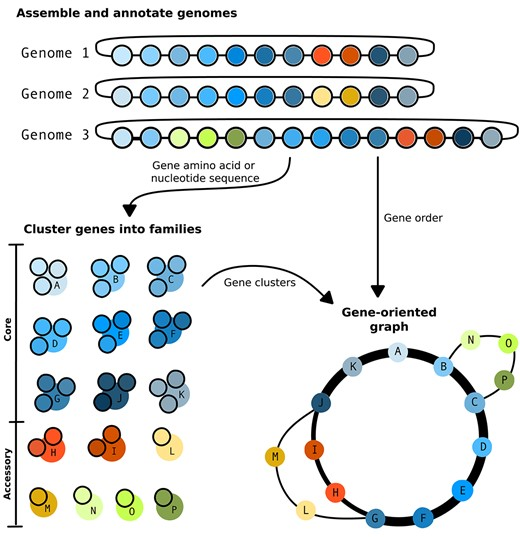
\includegraphics[width=0.8\linewidth]{images/graphePanFam.jpeg}
    \caption[Représentation d'un pangénome de gènes sous forme de graphe]{\textbf{Représentation d'un pangénome de gènes sous forme de graphe.} Extrait de \cite{matthews_gentle_2024}}
    \label{fig:graphPanFam}
\end{figure}

\subsection{Méthodes et outils de pangénome de gènes}

Le premier outil dédié à la construction de pangénomes de famille de gènes est Edgar \cite{blom_edgar_2009}. Disponible en ligne, ce n'est pas un outil à proprement parler, mais plutôt une ressource de résultats d'analyse de pangénome. Dans sa méthode, Edgar clusterise les gènes en familles d'orthologues, en utilisant le BBH\footnote{\textit{Bidirectional Best Hit}}. Les génomes étant relativement proches dans les analyses, les paralogues récents pourraient être regroupés avec des orthologues. Les familles sont donc raffinées en utilisant un système de score pour valider les BBH. Dans sa version actuelle, l'outil permet d'identifier le \textit{core genome} et l'\textit{accessory genome}, rechercher des synténies conservées, de construire des arbres phylogénétiques, ou encore d'annoter fonctionnellement les gènes à partir de bases de données de référence.

Le premier outil permettant la construction de pangénome en ligne de commande est PGAP \cite{zhao_pgap_2012}. Le premier intérêt de PGAP, est qu'il permet à l'utilisateur de construire un pangénome avec ses propres génomes. PGAP construit lui aussi des familles d'orthologues. À partir de ces familles, il propose différentes analyses, comme la courbe de raréfaction, le profil du pangénome\footnote{Le nombre de gènes (y) présents dans x génomes.}, l'identification du \textit{core genome}, l'analyse de variants. Une interface PGAP-X \cite{zhao_pgap-x_2018} rend l'outil plus accessible et améliore la visualisation des résultats.

PanOCT \cite{fouts_panoct_2012} est un autre outil disponible en ligne de commande. Il propose aussi un clustering en famille orthologues, similaire à EDGAR, mais améliore l'algorithme en ajoutant l'information de contexte conservé (\textit{Conserved Gene Neighborhood}, CGN). Les gènes orthologues ont tendance à conserver leur organisation génomique dans les espèces proches contrairement aux espèces éloignées et aux gènes paralogues \cite{huynen_measuring_1998,rocha_organization_2008}. En combinant le BBH et le CGN, les familles de gènes orthologues sont de meilleure qualité. L'outil PanACEA \cite{clarke_panacea_2018} récupère les familles de PanOCT et permet de visualiser le pangénome, mais aussi de l'annoter, notamment avec des informations liées à l'antibiorésistance. 

PanFunPro \cite{lukjancenko_panfunpro_2013}, propose une méthode originale pour construire des familles de gènes homologues, en se basant sur l'annotation fonctionnelle des protéines. Pour annoter les protéines, il utilise des profils HMM de différentes bases de données de domaines protéiques. En définissant l’homologie selon la fonction plutôt que la séquence, cette approche propose un cadre d’analyse alternatif, privilégiant les similarités fonctionnelles des protéines et offrant ainsi une vision complémentaire aux méthodes traditionnelles.

Roary \cite{page_roary_2015} est l'outil de pangénomique certainement le plus utilisé et le plus célèbre. Sa popularité vient de sa capacité à générer des pangénomes de façon rapide en demandant peu de ressources par rapport à ses concurrents de l'époque. Pour ça, il utilise un algorithme CD-Hit pour grouper les séquences proches avant d'aligner les séquences représentantes entre elles avec BLASTP. Les familles sont construites avec l'algorithme MCL et raffinées en utilisant les informations de colocalisation. Roary est aussi un des premiers programmes à représenter les pangénomes de gènes sous forme d'un graphe dans lequel les n\oe uds sont les gènes et les arêtes représentent une relation de voisinage dans les génomes.

\newpage
D'autres outils vont reprendre ce modèle de graphe de gènes, comme Panaroo \cite{tonkin-hill_producing_2020}. À partir du graphe, il corrige les erreurs d'annotation et d'assemblage. Il dispose également de plusieurs modules d'analyse : GWAS, SV, phylogénie et visualisation du pangénome. Panaroo est un outil performant, mais demande des ressources de calcul relativement importantes et une expertise bioinformatique plus importante que d'autres outils. De plus, en nettoyant le graphe, il est possible qu'il élimine des évènements évolutifs récents, et donc ne pas être adapté à des taxons dans lesquels les taux de HGT sont élevés par exemple. Panakeia \cite{beier_panakeia_2022} est un outil reposant aussi sur un modèle de graphe de pangénome, mais propose une analyse plus "universelle". L'outil propose entre autres l'identification de chemins particuliers dans le graphe, correspondant à des structures biologiques, comme les îlots génomiques.

Les outils présentés jusqu'ici, bien que non limités théoriquement, sont généralement appliqués à la construction de pangénomes au niveau de l'espèce. Des méthodes, comme RIBAP \cite{lamkiewicz_ribap_2024}, proposent de construire des pangénomes au niveau du genre. RIBAP construit un pangénome en utilisant ROARY à 95 \% d'identité. En parallèle, il utilise MMSeqs2 pour aligner l'ensemble des gènes. Le résultat de l'alignement est ensuite utilisé pour raffiner les familles pour construire des familles homologues au niveau du genre. De cette manière, la partie de \textit{core genome} est plus importante. Avec ce nouveau partitionnement, RIBAP propose de construire un arbre phylogénétique des souches présentes dans le pangénome. 

L'utilisation de pangénomes de gènes est bien adaptée à la génomique comparée des procaryotes. Leur simplicité de calcul et d'interprétation les rend accessibles pour tous les utilisateurs. Néanmoins, cette simplicité est liée à une vision gène centrée, qui ne prend pas en compte les régions non codantes. Des outils, comme Piggy \cite{thorpe_piggy_2018}, permettent de pallier ce problème en proposant une analyse complémentaire à un pangénome de gène généré par Roary. Ainsi, la complémentarité des outils permet d'avoir une étude plus complète. 

En 2020, PPanGGOLiN \cite{gautreau_ppanggolin_2020} introduit une stratégie de partitionnement, s’appuyant sur un algorithme de \textit{machine learning} pour classifier les gènes du pangenome. Cette approche repose sur une analyse des relations de voisinage et du clustering, éliminant ainsi la nécessité de fixer des seuils stricts. Par conséquent, PPanGGOLiN permet d’identifier de manière dynamique les trois composantes du pangenome — \textit{persistent genome}, \textit{shell genome} et \textit{cloud genome} — sans présupposer de leur répartition.

\subsection{Analyses à partir de pangénomes de gènes}

Les pangénomes de gènes sont utilisés pour mener des études de phylogénomique. En 2020, Gaba \textit{et al.} \cite{gaba_pan-genome_2020} s'intéressent aux archées de la classe des Halobacteria, des archées extrêmement halophiles\footnote{Capable de vivre dans des milieux à haute concentration en sel}. Ils vont construire un pangénome à l'aide de l'outil GET\textunderscore HOMOLOGUE \cite{contreras-moreira_get_homologues_2013}, un outil similaire à EDGAR. À partir de ce pangénome, ils ont pu identifier les gènes \textit{core} des gènes \textit{accessory}. Sur la base de ce partitionnement, ils ont pu mettre en évidence un fort taux de transferts horizontaux au sein de la classe des Halobacteria. Ils ont alors construit une phylogénie basée sur le pangénome et sa partition, mettant en évidence une évolution étroite entre l'ordre des Natrialbales et celui des Halobacteriales, suggérant alors l'existence d'un superordre les regroupant. Plusieurs méthodes permettent d’ailleurs d'identifier les régions où les transferts horizontaux de gènes se produisent préférentiellement. Parmi elles, la méthode panRGP\cite{bazin_panrgp_2020} permet de détecter les régions de plasticité génomique (RGP), \textit{i.e.} des segments du génome échangés entre différentes souches par transfert horizontal ou perdus de manière différentielle selon les lignées. Cette approche repose sur l’analyse du graphe de pangénome et de sa partition pour identifier les régions variables. Elle permet également d’identifier des spots, en repérant les familles de gènes persistantes flanquant les RGP. Une autre méthode, panModule\cite{bazin_panmodule_2021}, vise quant à elle à détecter des groupes de familles de gènes variables dans le pangénome, qui sont organisés en blocs de synténie au sein des génomes. Ces deux méthodes sont intégrées à la suite logicielle PPanGGOLiN et exploitent le graphe de pangénome généré par cette dernière.

Dans les exemples cités, les études étaient centrées sur des groupes taxonomiques et donc les génomes appartenaient au même taxon. Pourtant, comme nous l'avons déjà vu, l'étude d'environnements et les données métagénomiques sont étroitement liées aux études pangénomiques. Vera-Ponce de León \textit{et al.} \cite{vera-ponce_de_leon_genomic_2024}, produisent un atlas génomique du microbiote des saumons. Pour caractériser les espèces présentes et construire le pangénome, ils utilisent l'outil mOTUpan \cite{buck_motupan_2022}. mOTUpan permet de clusteriser les métagénomes à un fort niveau d'identité (95 \%), définissant ainsi des unités taxonomiques opérationnelles métagénomiques (mOTUs, \textit{metagenomic Operational Taxonomic Unit} en anglais). Chaque mOTU peut être associé à une espèce (ou un taxon) et donc permettre de séparer les gènes appartenant à la même espèce dans une même mOTU. L'intérêt de mOTUpan est qu'il utilise un modèle bayésien pour estimer le génome \textit{core} et le génome accessoire. Ce modèle prend en compte la complétion (souvent faible) des métagénomes et améliore la qualité du partitionnement sur ces données. À partir du pangénome, les auteurs ont pu identifier 14 ordres bactériens différents, représentant 35 genres distincts, ils ont également identifié 29 nouvelles espèces encore non répertoriées.

Les méthodes de machine learning peuvent aussi être utilisées pour analyser les pangénomes. Dans leur article, Kavvas \textit{et al.} \cite{kavvas_machine_2018} proposent d'utiliser des méthodes de machine learning pour identifier des gènes de résistance aux antibiotiques dans 1 595 souches de \textit{Mycobacterium tuberculosis}. Le pangénome est construit à partir de familles homologues, et les gènes connus pour être des gènes de résistance aux antibiotiques sont annotés. En utilisant des méthodes de machine learning (SVM, MI, ANOVA\dots), les auteurs ont pu identifier 24 nouveaux gènes de résistance, de plus le signal de certains gènes déjà connus est plus fort que mesuré précédemment. Les auteurs ont poursuivi en analysant la structure des nouveaux gènes et de leurs protéines, ainsi qu'en menant une étude géographique de la répartition des gènes pour établir des liens entre population hôte et résistance. Il faut néanmoins rappeler une nouvelle fois que la découverte de ces nouveaux gènes doit être vérifiée et que leur identification n'est possible que sur la base d'une base de données de gènes connus.

\begin{table}[htbp]
  \centering
  \footnotesize
  \begin{tabular}{|p{.2\textwidth}|p{.38\textwidth}|p{.35\textwidth}|}
    \hline
    Nom & Méthode & Référence \\
    \hline
    EDGAR & matrice présence/abscence & \cite{blom_edgar_2009}\\
    \hline
    PGAP & matrice présence/abscence & \cite{zhao_pgap_2012}\\
    \hline
    PanOCT & Clustering d'orthologue & \cite{fouts_panoct_2012}\\
    \hline
    GET\textunderscore HOMOLOGUES & Clustering d'orthologue & \cite{contreras-moreira_get_homologues_2013} \\
    \hline
    PanACEA & Visualisation & \cite{clarke_panacea_2018}\\
    \hline
    PanFunPro & Familles de profil fonctionnelle & \cite{lukjancenko_panfunpro_2013}\\
    \hline
    Roary & Graphe de famille de gène & \cite{page_roary_2015}\\
    \hline
    Piggy & Analyse région intergénique & \cite{thorpe_piggy_2018}\\
    \hline
    Ptolemy & Graphe de famille de gène & \cite{thorpe_piggy_2018}\\
    \hline
    PIRATE & Graphe de famille de gène & \cite{bayliss_pirate_2019}\\
    \hline
    Panaroo & Graphe de famille de gène & \cite{tonkin-hill_producing_2020}\\
    \hline
    PPanGGOLiN & Graphe de famille de gène & \cite{gautreau_ppanggolin_2020}\\
    \hline
    PanACoTA & Graphe \& Phylogénie & \cite{perrin_panacota_2021} \\
    \hline
    Panakeia & Graphe de famille de gène & \cite{beier_panakeia_2022}\\
    \hline
    PanPhlAn & Graphe de données métagénomique & \cite{scholz_strain-level_2016}\\
    \hline
    MSPminer & Graphe de données métagénomique & \cite{plaza_onate_mspminer_2019}\\
    \hline
    mOTUpan & Graphe de données métagénomique & \cite{buck_motupan_2022}\\
    \hline
    Pan-Tetris & Visualisation & \cite{hennig_pan-tetris_2015}\\
    \hline
    PanViz & Visualisation & \cite{pedersen_panviz_2017}\\
    \hline
    Panache & Visualisation & \cite{durant_panache_2021}\\
    \hline
    
  \end{tabular}
  \caption[Outils de pangénomique basés sur les familles de gènes]{\textbf{Liste non exhaustive d'outils de pangénomique basés sur les familles de gènes}}
  \label{tab:pangenomicToolsFam}
\end{table}

\newpage
\section{Conclusion sur les pangénomes et éléments de réflexions}

Nous avons présenté une grande variété de méthodes et d'outils de pangénomique (\textit{cf.} tableaux \ref{tab:pangenomicToolsSeq} et \ref{tab:pangenomicToolsFam}) et exploré plusieurs champs d'application des pangénomes. Cependant, plusieurs défis majeurs restent à relever en pangénomique.

Un premier défi concerne la représentation et la visualisation des pangénomes. En effet, ceux-ci doivent être visualisables par l'\oe il humain tout en intégrant l’ensemble de l’information génomique. Différentes approches ont été développées pour répondre à cette problématique, notamment des outils de visualisation interactifs. À titre d’exemple, Pan-Tetris\cite{hennig_pan-tetris_2015} permet de visualiser et de modifier la composition des groupes de gènes grâce à une technique inspirée du jeu Tetris. PanViz\cite{pedersen_panviz_2017} facilite la comparaison des génomes individuels aux pangénomes avec une navigation basée sur l'ontologie des gènes. PanVa\cite{van_den_brandt_panva_2024}, utilisant les pangénomes de PanTools\cite{sheikhizadeh_pantools_2016}, propose une approche centrée sur la variabilité structurale, permettant une analyse flexible des pangénomes en tenant compte des variations génomiques complexes. Enfin, PANACHE\cite{durant_panache_2021} propose une visualisation linéarisée des pangénomes, affichant la présence ou l’absence des blocs de séquences sous forme de navigateur génomique.

Un second défi crucial est celui du stockage et de la gestion des données pangénomiques. Contrairement aux génomes individuels, généralement stockés sous forme de texte et reliés à des bases de données, les pangénomes sont des structures plus complexes qui ne peuvent être stockées sous un format linéaire. Les BD doivent donc permettre un accès rapide et efficace aux informations, tout en étant mises à jour régulièrement pour suivre l’augmentation du volume des données génomiques. Des BD comme panKB \cite{sun_pankb_2025}, permettent d'avoir accès à des informations sur des pangénomes précalculés, reliés à des métadonnées comme les publications de références, les informations sur l'origine des génomes\dots Cependant, le pangénome en lui-même n'est pas disponible et seuls les résultats d'analyse sont disponibles.

Enfin, un défi essentiel concerne la construction du pangénome. Le choix des méthodes influence fortement le résultat final, mais les données d’entrée jouent également un rôle fondamental. L’objectif étant de représenter au mieux la diversité génomique, il est important de maximiser cette diversité tout en évitant les biais, tels que la surreprésentation de génomes pathogènes dans les bases de données. Un équilibre est nécessaire : trop de variations dans les données d’entrée peuvent complexifier l’analyse, en rendant par exemple les graphes de pangénome difficilement exploitables. La qualité des génomes, des annotations et des bases de données est également un facteur déterminant pour garantir la robustesse des analyses pangénomiques.

Pour répondre à ces défis, les méthodes et les outils de pangénomique sont en constante évolution. Avec ces progrès, divers domaines de la microbiologie voient progressivement s'intégrer des analyses pangénomiques en routine. Cette intégration repose en partie sur des plateformes qui rendent ces outils accessibles et exploitables par la communauté scientifique. Par exemple, MicroScope\cite{vallenet_microscope_2020} permet de construire des pangénomes procaryotes à l’aide de PPanGGOLiN \cite{gautreau_ppanggolin_2020} et d’identifier les régions de plasticité génomique (RGP) grâce à la méthode panRGP\cite{bazin_panrgp_2020}. MicroScope constitue alors un point entre les données génomiques, la production de pangénomes et leur utilisation effective, contribuant ainsi à relever progressivement les défis liés à la visualisation, au stockage et à la construction des pangénomes.

% \begin{table}[htbp]
%     \centering
%     \footnotesize
%     \begin{tabular}{|p{.25\textwidth}|p{.15\textwidth}|p{.35\textwidth}|p{.25\textwidth}|}
%         \hline
%         Nom & Type de pangénome & Méthode & Référence \\
%         \hline
%         NGSPanPipe & Séquence & Séquence représentative & \cite{kulsum_ngspanpipe_2018} \\
%         \hline
%         Spine & Séquence & Séquence représentative & \cite{ozer_characterization_2014}\\
%         \hline
%         VG toolkit & Séquence & Variant prédéterminé & \cite{garrison_variation_2018} \\
%         \hline
%         Minigraph & Séquence & Variant prédéterminé & \cite{li_design_2020} \\
%         \hline
%         PanVC & Séquence & Variant prédéterminé & \cite{norri_founder_2021} \\
%         \hline
%         Minigraph-Cactus & Séquence & MSA & \cite{hickey_pangenome_2024}\\
%         \hline
%         Harvest & Séquence & MSA & \cite{treangen_harvest_2014} \\
%         \hline
%         PGGB & Séquence & MSA & \cite{garrison_building_2024}\\
%         \hline
%         Cortex & Séquence & graphe de De Bruijn & \cite{iqbal_novo_2012} \\
%         \hline
%         Bifrost & Séquence & graphe de De Bruijn & \cite{holley_bifrost_2020} \\
%         \hline
%         SplitMEM & Séquence & graphe de De Bruijn & \cite{marcus_splitmem_2014} \\
%         \hline
%         PanTools & Séquence & graphe de De Bruijn & \cite{sheikhizadeh_pantools_2016} \\
%         \hline
%         twoPaCo & Séquence & graphe de De Bruijn & \cite{minkin_twopaco_2017}\\
%         \hline
%         DBGWas & Séquence & graphe de De Bruijn & \cite{jaillard_fast_2018}\\
%         \hline
%         EDGAR & Gènes & matrice présence/abscence & \cite{blom_edgar_2009}\\
%         \hline
%         PGAP & Gènes & matrice présence/abscence & \cite{zhao_pgap_2012}\\
%         \hline
%         PanOCT & Gènes & Clustering d'orthologue & \cite{fouts_panoct_2012}\\
%         \hline
%         GET\textunderscore HOMOLOGUES & Gènes & Clustering d'orthologue & \cite{contreras-moreira_get_homologues_2013} \\
%         \hline
%         PanACEA & Gènes & Visualisation & \cite{clarke_panacea_2018}\\
%         \hline
%         PanFunPro & Gènes & Familles de profil fonctionnelle & \cite{lukjancenko_panfunpro_2013}\\
%         \hline
%         Roary & Gènes & Graphe de famille de gène & \cite{page_roary_2015}\\
%         \hline
%         Piggy & Gènes & Analyse région intergénique & \cite{thorpe_piggy_2018}\\
%         \hline
%         Ptolemy & Gènes & Graphe de famille de gène & \cite{thorpe_piggy_2018}\\
%         \hline
%         PIRATE  & Gènes & Graphe de famille de gène & \cite{bayliss_pirate_2019}\\
%         \hline
%         Panaroo & Gènes & Graphe de famille de gène & \cite{tonkin-hill_producing_2020}\\
%         \hline
%         PanACoTA & Gènes & Graphe \& Phylogénie & \cite{perrin_panacota_2021} \\
%         \hline
%         Panakeia & Gènes & Graphe de famille de gène & \cite{beier_panakeia_2022}\\
%         \hline
%         PanPhlAn & Gènes & Graphe de données métagénomique & \cite{scholz_strain-level_2016}\\
%         \hline
%         MSPminer & Gènes & Graphe de données métagénomique & \cite{plaza_onate_mspminer_2019}\\
%         \hline
%         mOTUpan & Gènes & Graphe de données métagénomique & \cite{buck_motupan_2022}\\
%         \hline
%         Pan-Tetris & Gènes & Visualisation & \cite{hennig_pan-tetris_2015}\\
%         \hline
%         PanViz & Gènes & Visualisation & \cite{pedersen_panviz_2017}\\
%         \hline
%         PanVA & Sequence & Visualisation & \cite{van_den_brandt_panva_2024} \\
%         \hline
%         Panache & Gènes & Visualisation & \cite{durant_panache_2021}\\
%         \hline
        
%     \end{tabular}
%     \caption[Outils de pangénomique]{Liste non exhaustive d'outils de pangénomique}
%     \label{tab:pangenomicTools}
% \end{table}